\section{PicoBlazer}
\subsection{Flags}
\begin{enumerate}[nosep]
	\item Zero Z
	\item Carry C
	\item Overflow V
	\item Negative N
\end{enumerate}


\subsection{Addressbereiche}
\todo{Zeige Instruktionen welche in jeweilige Bereich schreiben kann.
% TODO: \usepackage{graphicx} required
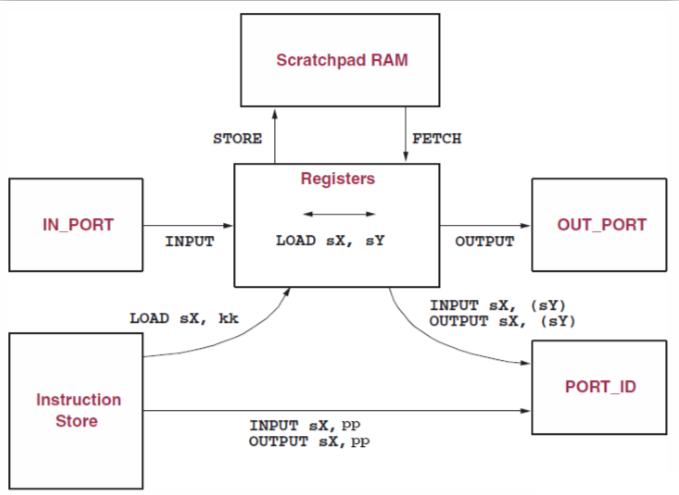
\includegraphics[width=\columnwidth]{Images/datamovement}
}
\begin{enumerate}[nosep]
	\item Instruction PROM, ProgramFlowControl
	\item General-Purpose Register, Moving Data
	\item Scratchpad RAM, Moving Data
	\item I/O Port, Moving Data
	\item CALL/RETURN Stack, ProgramFlowControl
\end{enumerate}

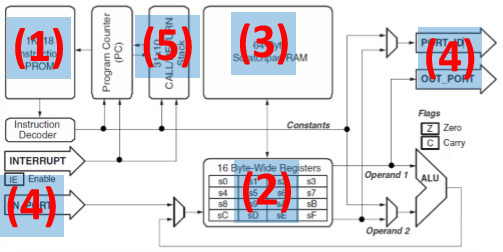
\includegraphics[width=\columnwidth]{Images/addressranges}


\subsection{Asynchrone Events}
\subsubsection{IRQ Event}
Ein IRQ-Event ist ein asynchrones Event, welches zu einer Unterbrechung des normalen Programmablaufs führen \textit{kann}. Der Ablauf in der Hardware ist wie folgt definiert:
\begin{lstlisting}
// (0) only respond to IRQ input if IE flag is set, i.e. after EINT or RETI ENABLE instruction
if ((IE = 1) and (IRQ input = HIGH)) {
	// (1) clear the IE FLAG
	IE <- 0
		
	// (2) push	the current PC to top of stack (TOS). Return Value
	TOS <- PC
		
	// (3) preseve flags
	PRESERVED_CARRAY <- CARRY
	PRESERVED_ZERO <- ZERO
		
	// (4) load PC with IRQ-Vec
	PC <- $3FF
}
\end{lstlisting}

\subsubsection{RESET Event}
Ein RESET-Event ist ein asynchrones Event, welches zu einem Neustart der CPU führt. Dies löscht die Register und ScratchPad RAM \underline{nicht}! Der Ablauf in der Hardware ist wie folgt definiert:
\begin{lstlisting}
// (0) only respond if priority is high
if (RESET input = HIGH) {
	// (1) Clear PC
	PC <- 0
	
	// (2) disable IRQ
	IE <- 0
		
	// (3) Reset flags
	CARRY <- 0
	ZERO <- 0
}
\end{lstlisting}